%
% The MIT License (MIT)
%
% Copyright (c) 2017 Paul Batty
%
% Permission is hereby granted, free of charge, to any person obtaining a copy
% of this software and associated documentation files (the "Software"), to deal
% in the Software without restriction, including without limitation the rights
% to use, copy, modify, merge, publish, distribute, sublicense, and/or sell
% copies of the Software, and to permit persons to whom the Software is
% furnished to do so, subject to the following conditions:
%
% The above copyright notice and this permission notice shall be included in
% all copies or substantial portions of the Software.
%
% THE SOFTWARE IS PROVIDED "AS IS", WITHOUT WARRANTY OF ANY KIND, EXPRESS OR
% IMPLIED, INCLUDING BUT NOT LIMITED TO THE WARRANTIES OF MERCHANTABILITY,
% FITNESS FOR A PARTICULAR PURPOSE AND NONINFRINGEMENT. IN NO EVENT SHALL THE
% AUTHORS OR COPYRIGHT HOLDERS BE LIABLE FOR ANY CLAIM, DAMAGES OR OTHER
% LIABILITY, WHETHER IN AN ACTION OF CONTRACT, TORT OR OTHERWISE, ARISING FROM,
% OUT OF OR IN CONNECTION WITH THE SOFTWARE OR THE USE OR OTHER DEALINGS IN
% THE SOFTWARE.
%

\section{Architecture}

Now that the paper has covered all the concepts and ideas needed to build a full continuous deployment pipeline, this next section aims to look at the different forms found in use and how they are put together.

\subsection{Starting point}

So far the paper has mentioned a pipeline, the pipeline will take the developers changes and pass them out to the user in working order. From a purely simplistic point of view the pipeline will look like the that seen in figure \ref{fig:pipeline-simple}.

\begin{figure}[H]
	\centering
	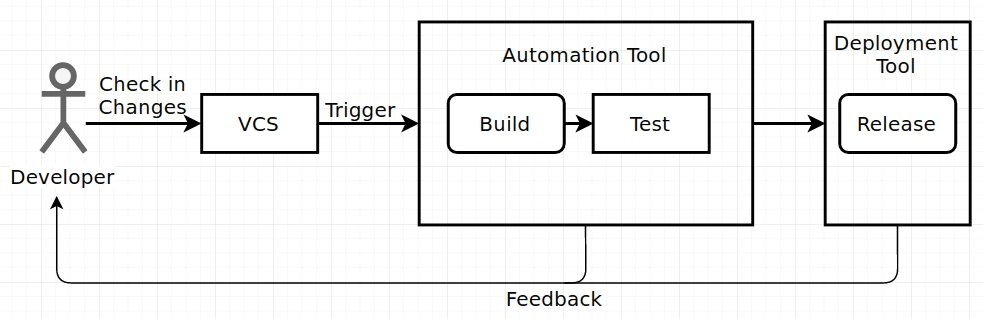
\includegraphics[scale=0.45]{images/pipeline-simple.jpg}
	\caption{The pipeline made simple}
	\label{fig:pipeline-simple}
\end{figure}

The developer will check in the code to the VCS which in turn will trigger the automation tool. The automation tool will then build the project and test, before sending it out to be released, placing it in the users hands. If any of the stages fail the rest of the pipeline is not ran and feedback is sent to the developer so they can fix it, or anyone else interested in the status of the project. 
\\\\
The testing part of the pipeline refers to unit tests and the other forms mentioned in the earlier chapters. Even if the system does successfully pass the feedback will still be sent, this will help guard against false positives.
\\\\
When talking about the architecture of such a system there are two side, firstly the software pipeline as seen above. How each of the steps flow into each other and what is needed to pass between each of the steps. The second is the hardware layout,  such as are the unit tests ran on the same server that it is built on, or maybe the entire pipeline in confined to a single server.

\subsection{Software architecture}
\label{sec:testing}

Figure \ref{fig:pipeline-simple} showed a basic pipeline for a continuous delivery pipeline, however there is not enough details to build a system from this. Below figure \ref{fig:bsipipeline} shows the system developed for the project that sparked this paper:

\begin{figure}[H]
	\centering
	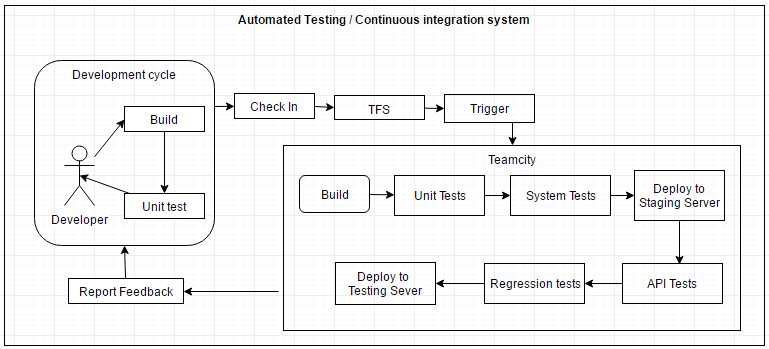
\includegraphics[scale=0.6]{images/bsipipleine.png}
	\caption{A full delivery pipeline}
	\label{fig:bsipipeline}
\end{figure}

The figure shows two things, firstly it reveals the local development cycle. The cycle being that the developer will check the basics before checking in the code to the VCS in this case a TFS server. Not noted on the diagram the developer will also have access to a local running copy of the program allowing them to run other forms of tests if needed. 
\\\\
The second part, it expands on the build and test block previously seen, firstly, the build, then the unit tests followed by system tests. System tests not mention before are a form of integration tests. This then leads onto an interesting part where the system is deployed onto a staging instance, this allows the API and regression tests to be ran, as they require the system to be up and running. This is then deployed to testing  for manual tests, where it can then be pushed to production. In continuous deployment theses steps would be automated.
\\\\
The interesting part here is how four different deployments are needed, one for the developer, one for staging, one for testing and one for production. This is where Docker and other such tools fit into the picture.
\\\\
This kind of pipeline is a common one, some may use different types of tests as it will suite their needs better, but the theme is still the same. One such system by \cite{zend} adds an additional step after build to package the system up, ready to deploy, and as mentioned they have swapped out the test types for that which suit their product.
\\\\
Another interesting take on this by \cite{codeahoy}, has split their project into different components, this means rather than having one project to handle integration tests, both systems have to be built and then integrated together. Therefore they used the architecture in figure \ref{fig:codeahoy}:

\begin{figure}[H]
	\centering
	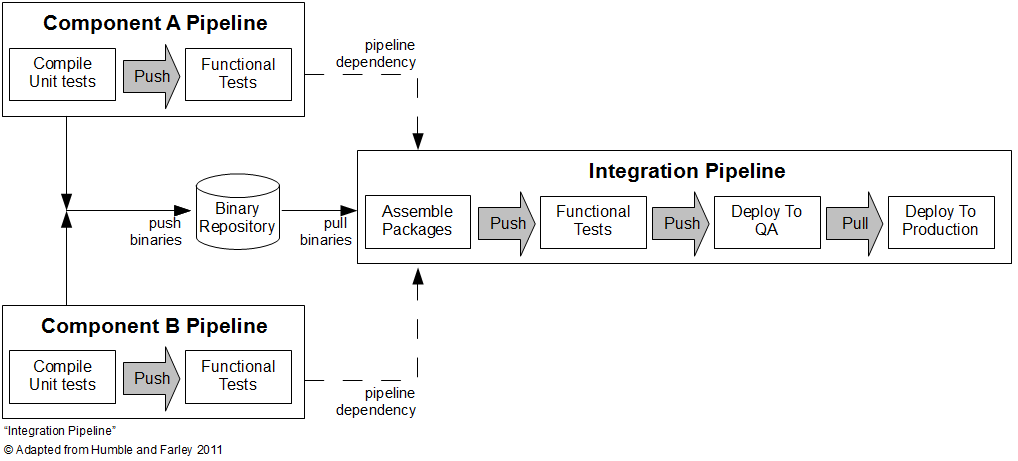
\includegraphics[scale=0.5]{images/codeahoy.png}
	\caption{A dual channel delivery pipeline by \cite{codeahoy}}
	\label{fig:codeahoy}
\end{figure}

This design has added an additional repository for binaries, then when a commit is placed in component A or B, it can progress through the entire pipeline by getting the latest version of the other components binaries from the repository. 
\\\\
\cite{thoughworks} takes this a step further by not only splitting the pipeline into separate components  but also places them in different repositories, making the first time they are integrated together being the integration tests as they all come from their own binary repositories.
\\\\
This kind of pattern goes along with the development environments based on breaking up a monolithic architecture  into smaller more manageable or modular units. This system makes it easy to add continuous deployment into a micro service or other types of modular architecture.
\\\\
One thing not shown so far but some teams find invaluable is to run a static analysis on the code base to pre-emptively spot erroneous areas in the project before they happen. This can then be sent back with the rest of the report to the developers and other interested parties.
\\\\
This basic pattern and flow of the pipeline does seems to be a common theme throughout all implementations.  With the single monolith structure taking it from the start to end and the second combining multiple components into a single software package. 

\subsection{VCS workflow}
\label{sec:vcs}

As seen the pipeline is generally triggered via a commit into the VCS this makes the workflow with the branch structure and VCS a central component into how the rest of the systems are put together.
\\\\
There are two main schools of thoughts when working with continuous deployment and VCS the first is more commonly seen in open source projects that are hosted on sites such as Github and Bitbucket, with the second when everyone has full access to the repository. 
\\\\
The first uses a pull request system, all the developers or contributors to the project will submit their changes through a pull request. When the request is made an automated system will start the process of running through the pipeline. 
\\\\
Here the system can automatically merge the change if it passes, however, in open source project it is more common to find the owners performing a code review and checks for harmful changes before merging the request manually. If however it is a private repository the code checked in can be automatically merged. 
\\\\
If the checks fail the request can remain open until an update is pushed to it where it will run the checks again. This is visualised in figure \ref{fig:osspipeline}.

\begin{figure}[H]
	\centering
	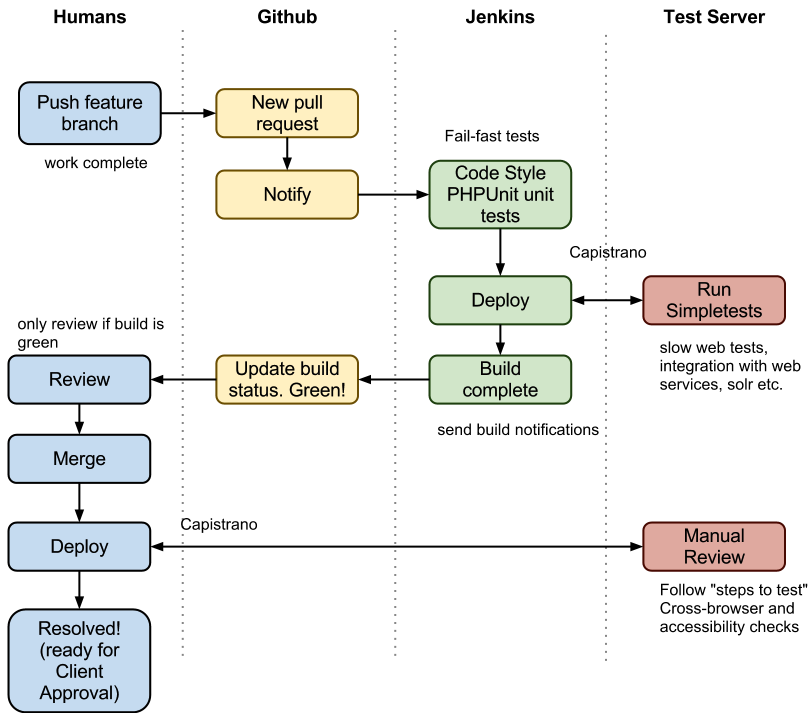
\includegraphics[scale=0.4]{images/osspipeline.png}
	\caption{Pull request delivery pipeline by \cite{osspipeline}}
	\label{fig:osspipeline}
\end{figure}

The only thing to note about the diagram is the manual review as mentioned, this could be automated creating the full continuous delivery pipeline rather than continuous integration.
\\\\
The second system is similar to the pull request however rather than preforming the change in a pull request the commit is placed inside the teams VCS workflow branch. When working in a agile and continuous delivery environment it is generally accepted that there should be a master branch that is the latest version of the software. This is also the branch where all the development goes and what the customer gets.
\\\\
Following that system the main branch will have the pipeline attached, when a milestone is reached such as the end of a sprint in agile methodology. A new branch is created to represent the milestone at that point in time. 
\\\\
One reason for this workflow is it will carry well across multiple systems as TFS does not branch in the same way that GIT does. Branching in GIT is similar to changing the entire repository, for example if the current branch is master, then when changing to \textit{feature\_one} branch it is like renaming the folder and swapping its contents. Think of it like a magic room that changes depending on what branch it is on. TFS on the other hand has branches located on a different path, so rather than a single magic room, its will create a new room for each branch.
\\\\
This difference in design will affect how the automation tool will interact with the VCS, as if it is developed using GIT, the system can watch multiple branches at the same time as it is all located in the same place. Whereas with TFS a new configuration will have to be made for each branch as they are separate from each other.
\\\\
With this in mind, if the workflow used is to create a new branch per version work on it until release then repeat, at the end of every release a new configuration will have to be made for the new branch. While this does not vary from the other workflow in terms the amount of branching, new configurations will not have to be made as they will also be branched off with the project as seen in the next part. But, as development is performed on a single branch there is nothing to change until the project does.
\\\\
Before delving into the why a new configuration is not needed, the master branch of the project as defined must always be in working condition ready to be delivered the users. If commits are therefore placed directly in master and they make the build or tests fail, then the entire concept of continuous deployment has failed as master is not in a  production ready state.
\\\\
In order to combat this the preferred workflow is to use a feature branches, similarly to that of a pull request system, development is performed on another branch then when ready can be merged into the master. Similarly this allows tests and other action to be perform on the changes before they are merged into master. This assures that the master branch will be kept in a working condition.
\\\\
This will also allow the merge to be reverted if there is an issue in the integration without losing the work performed as more commits can be made, tested and merged again.
\\\\
Now that there is a workflow in place and the pipeline is ready to be attached to the branches, where does the code and other parts needed in the pipeline go. The tools such as Jenkins, Teamcity and CruiseControl all offer the ability to store scripts inside their systems through their user interface.
\\\\
For example Teamcity comes with pre-scripted runners that will allow a click and select experience to get the entire system set-up. While this is certainly a good selling point for non-experienced or quick one time set-ups over the long term this could be quite the opposite. In multiple ways, if the team decides they want to change from Teamcity to Jenkins now the entire system has to be built from the ground up. Otherwise it might end up trying to fit the way Teamcity handles things into Jenkins.
\\\\
Other issues with software versions, setting up new branches and language compatibility, there are many more reasons as to why it is good in the short term on small project but for larger and more longer terms a better system is needed.
\\\\
Rather than storing the scripts inside of the tool, they should be placed inside of the VCS then depending on the set up, the tool will just have to call a single or multiple external scripts, even if the scripts are a single line. In an ideal situation the scripts should be able to run on the target platforms for the project, such as using python or ruby rather than bash and batch, to save writing them twice.
\\\\
This also has the benefits of allowing someone to walk up to a brand new machine get the repository and have the full system up and running within minutes as the VCS holds all the scripts needed.

\subsection{Hardware architecture}

Up to this point the paper has focused on the software side of things looking at the pipeline, VCS and scripts. This next section will look at where this is hosted and how where each part can be split.  
\\\\
Firstly, the set-up will depend on the size of the team and number of builds being performed at once, for example a single server will be fine for small teams of five whereas when dealing with hundreds the servers also need to scale to match.
\\\\
At the minimum a single server is required, this will hold the VCS, automation tool and staging / testing instance. Finally it will have to include the deployment manager. In general this is a lot of work to place onto a single box and to expect quick feedback timings.
\\\\
Going back to the start of this paper on how automation tools work, the general principle is the central server and lots of registered agents that can take jobs from the sever. This leads nicely into the following architecture seen in figure \ref{fig:bamboo}:

\begin{figure}[H]
	\centering
	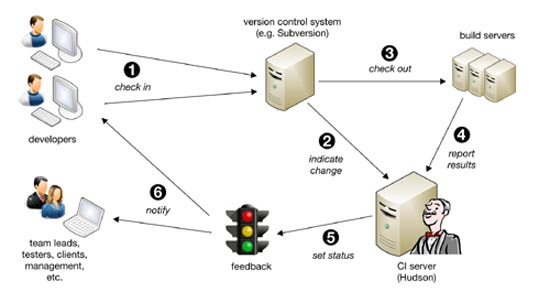
\includegraphics[scale=2.5]{images/bamboo.jpg}
	\caption{Server setup by \cite{bamboo}}
	\label{fig:bamboo}
\end{figure}

The figure shows that rather than having a single sever it is split into three parts, the first containing the VCS, the second the CI / automation tool, and the third a number of machines to perform the builds and tests as necessary.
\\\\
When the build severs are at max capacity new servers can be spun up registered to the automation tool ready to go. This creates a easily scalable solution that can also be downsized if needed.
\\\\
The main issues with this set-up is that some of the build servers may become specialised. While there may be twenty build servers one may be used for build in Linux this creates a bottleneck in the system, ideally all servers should be able to accomplish all the tasks, looking towards Docker or similar programs again for the solution. In order to try and reduce dependency on the machines  and the programs, creating an environment where the system can run on anything quickly.
\\\\
For web application this is generally not a problem as the build servers can be set up in way  that is appropriate and reflect the production environment, unless the application is designed to work across different servers such as Linux and Windows. This however is not the same for other types of development such as embedded systems.
\\\\
\cite{intel} has designed a work around, interestingly it uses the same principles as Docker, install once and run everywhere, however rather then dealing with software they have recommended to build a software emulator to emulate the target hardware. This emulation can then be ran on any machine allowing the once specialise system to be generalised over multiple servers, removing the bottleneck. This designed can be seen in figure \ref{fig:intel}:

\begin{figure}[H]
	\centering
	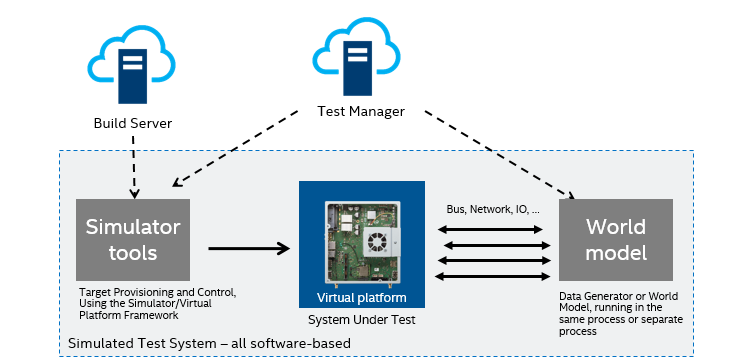
\includegraphics[scale=0.7]{images/intel.png}
	\caption{Embedded systems from \cite{intel}}
	\label{fig:intel}
\end{figure}

While this design works by abstracting the hardware platform into software, there is a large issue with the amount of effort required in order to create this emulation. This may be proprietary hardware or otherwise increasing the difficulty of such a task. There is also the issue with performance as it is now software rather then running directly onto the hardware. 
\\\\
In this part most of the solutions are focused on self-hosted and run solutions, however there is also the option to rent or buy the whole package rather then run them internally. For example, GihHub, BitBucket and GitLab provide a was to host GIT repositories, at a price, they even offer intergeneration with CI services such as Travis. 
\\\\
Cloudbees, BitbucketPipelines and others offer a cloud solution to take the repository and perform the operations on then removing the need to worry about servers and interaction between them. Ultimately the choice of system will come down to the project and budget at hand. With sensitive data, a self-hosted solution will work out better whereas a open source project will fair well with the cloud solutions.
\\\\
While the cloud solutions remove the need for handling the severs and sever set up themselves, the architecture discussed in this section will still apply as there will still be a need for a VCS server and automation tool server, it is just a matter of not dealing with them directly, but rather through a third party.

\subsection{Deployment}
\label{sec:deployment}

Up until this point the paper has covered all the parts within the pipeline apart from deployment, and how to deploy a system from the end of the pipeline. This next part aims to cover this.

\subsubsection{Databases}
Sometimes no matter what application it will have some form of database in the background, when the application updates, so does the database, changing the schema, tables or data types. In a continuous delivery pipeline this could happen multiple times in a day, whist trying to hold to the zero downtime expectations
\\\\
\cite{updatedatabse} has designed an application that achieves just that on a small scale, the paper also lists several alternatives that try and accomplish this. This is an on going area of research and should be expanded on to get the process to be as smooth as possible without disrupting the running of the application.  

\subsubsection{Servers}

Servers are unique as in general the company creating the product will also host or manage the server, this creates an easy situation where the entire pipeline is an internal process with minimal external needs, such as with the server company like Amazon web services (AWS).
\\\\
With a standard set-up the new version should be deployed behind the scenes then once done so the live site should now direct the the newer version rather than the old. This can create an easy fallback system if something goes completely wrong.
\\\\
The can be done by setting up another Docker container, or however the application is designed to be deployed, it is key however to have this automated. With regards to the database, ideally the database should be handled separately from the rest of the application to minimise errors. And when falling back to not have data loss.
\\\\
The deployment of servers are the type to be handled by the likes of Octopus, Chef and Puppet. That is not to say that they cannot be used for other type of deployment, more so that is where they are specialised.

\subsubsection{Downloadable applications}

As far as downloadable application or desktop applications, there are multiple options open, the main idea is to provide a area that can be checked and downloaded via the software, by bundling the software up. On Linux type operating systems (OS) this is normally checking in the bundled software in to the package control repository, and updated via the system package manager such as apt-get or Pacman. 
\\\\
However, on a Windows like OS, even possible on Linux there are multiple options open to handle the updating of software \cite{deploy} covers this, the final choice will come down to the type of software that is being deployed, a web browser can update and install in the background without the users knowledge fine, however more critical software must not, and must be handled with great care.

\subsubsection{Mobile applications}

Similarly, to Linux like application there is normally a gatekeeper in the way of pushing update directly to the user and instead must go through the "store". Therefore the deployment stage will consist of packaging the software up and submitting it to the store. 
\\\\
The ability to automate this process is not so much down to the software but rather the gatekeeper, as they may have manual review and delayed times between submissions, while internally continuous deployment can be used the gatekeeper may make it impossible to do so all the way to the user.

\subsection{Architecture final thoughts}

Overall, there are some very clear structures and patterns to be found when creating a continuous deployment system. Starting with the pipeline, emerging two main styles depending on the type of application.
\\\\
To the workflow around the pipeline ensuring that there is a master branch that is always in development and the practises around them. Either through the uses of a pull request or feature branch system.
\\\\
Then onwards to the hardware and server set with the ideal three tier set up, allowing easy expansion and reduction of servers as needed. Ensuring that each of the servers are generalised as to be able to run any task. Even those on specialised hardware. Including the opportunity to use other hosted services.
\\\\
Following on to the best practises around the deployment of the system for three different types of applications, web, downloadable and mobile.  
\\\\
While the final project may vary from depending on what part are used, the core principles, design and workflow found here should be used as the backbone of creating a continuous delivery or continuous integration system.